\documentclass[12pt]{article}
\usepackage{enumerate}
\usepackage{amsmath}
\usepackage{amssymb}
\usepackage{amsthm}
\usepackage{etoolbox}
\usepackage{graphicx}

\newcommand{\Name}[1]{\noindent \textbf{Name:} #1 \\}
\newcommand{\Workedwith}[1]{\noindent \textbf{Worked with:} #1 \\}
\newcommand{\Problem}[3]{\mbox{} \newline \noindent \textbf{\textbf{Problem #1: #2 [#3 Points] \\ }}}


\begin{document}

\begin{center}
  \bf
  Algorithms \\
  CMPT 307 D200 \\
  Spring 2024 \\
  \rm
  Homework 5\\
  Due:  Sunday, Mar 31 at 10:00 PM \\
\end{center}

\Name{Your name here}
\Workedwith{Everyone you worked with here}

\Problem{5}{Gamesville}{20}

Many puzzles can be solved by transforming (or ``reducing'') them to network flow problems.  That's what you'll do here, like the last problem!

A different popular online gaming website, Gamesville, has a puzzle on their website called Defective Chess Boards. DCB is a puzzle that goes like this:  We're given an $n \times n$ chessboard in which some cells are missing.  The goal is to tile the board with dominoes, each of which covers exactly two adjacent cells, or determine
that no such tiling exists.  Figure~\ref{fig:dominoes} shows a defective chess board and a valid tiling.  Describe an algorithm for determining whether or not a given $n \times n$ defective chess board has a valid tiling and, if it does, to find that tiling.  Prove
that your algorithm is correct and give its running time as a function of $n$.  You should assume that the input defective chess board is given to us as an $n \times n$ matrix where each entry in the matrix indicates if the corresponding cell in the board is black, white, or missing.

\begin{figure}[h]
\begin{center}
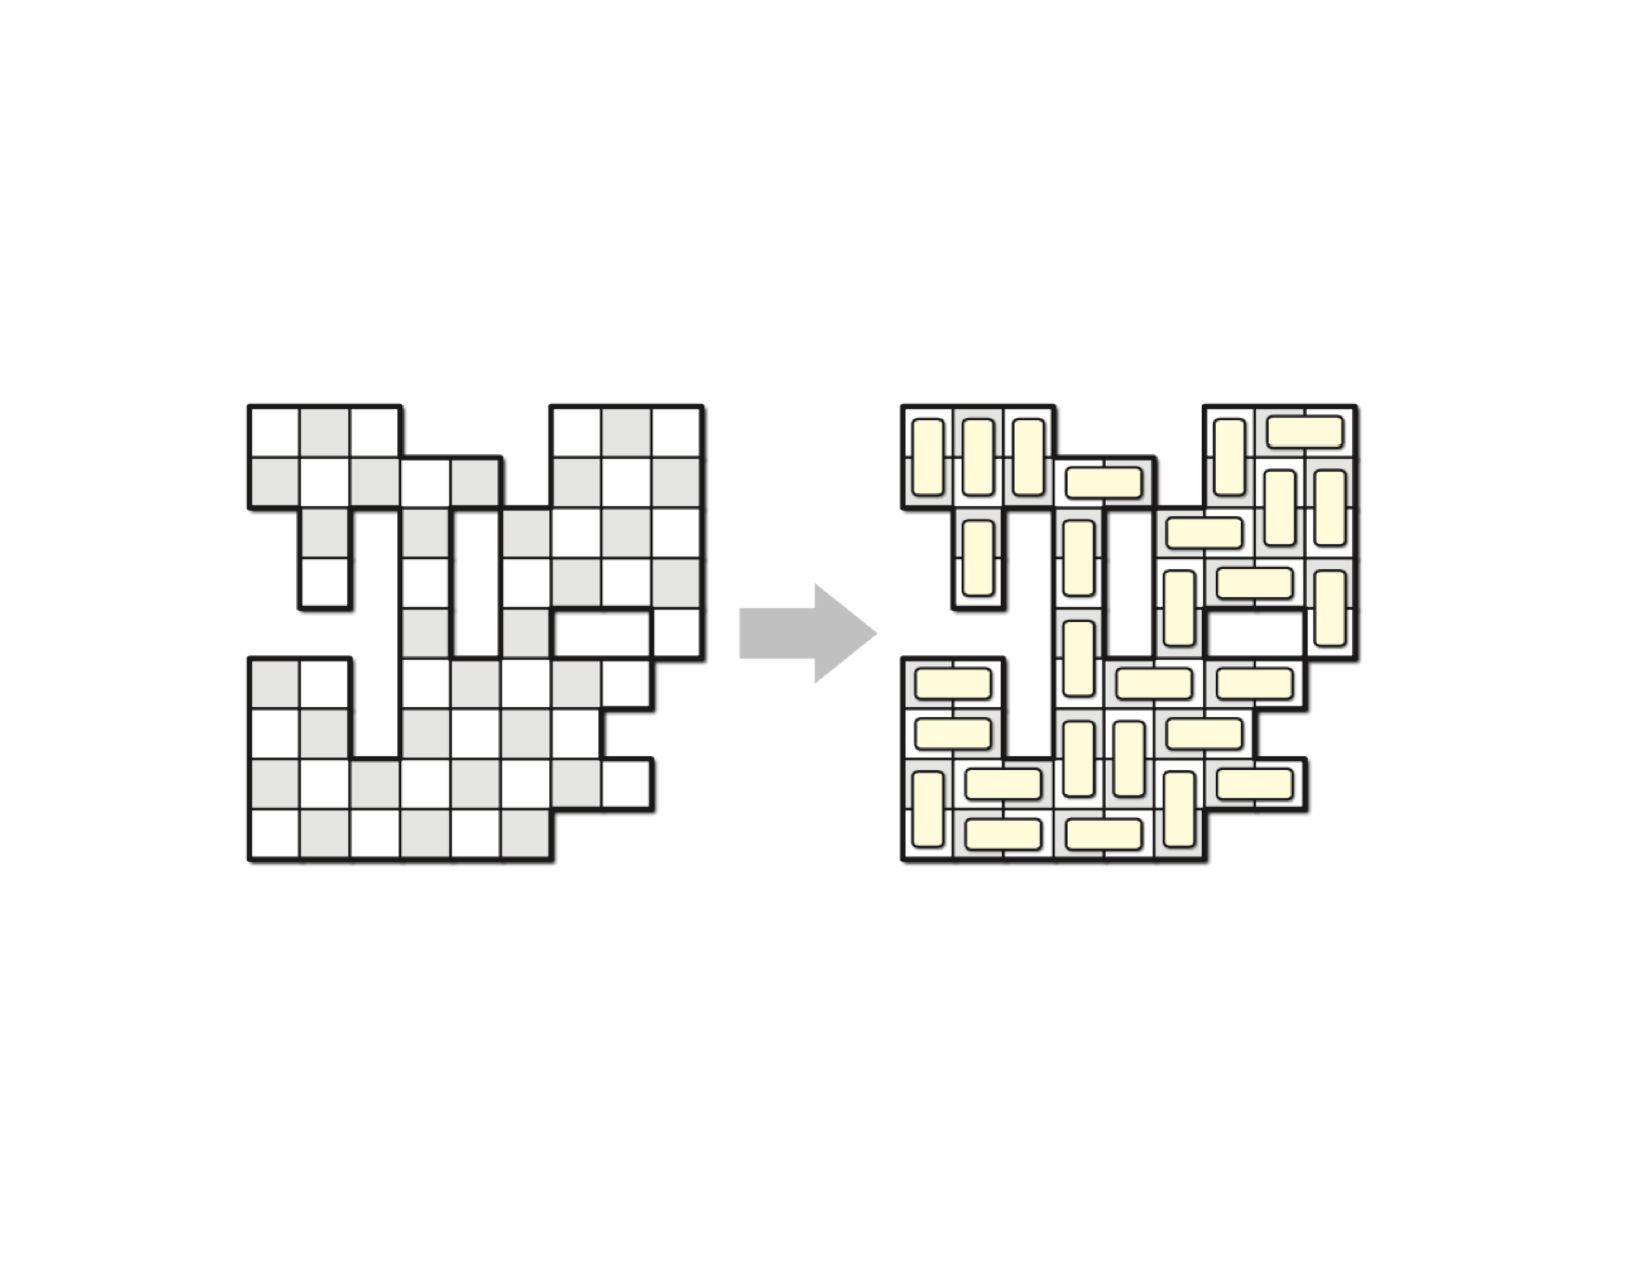
\includegraphics[width=4in]{Dominoes.pdf}
\end{center}
\caption{A defective chessboard and a tiling of that board with dominoes.}
\label{fig:dominoes}
\end{figure}

\textbf{Solution:}
% SOLUTION GOES HERE


\end{document}
